\documentclass[11pt,a4paper]{article}
\usepackage[utf8]{inputenc}
\usepackage[T1]{fontenc}
\usepackage{amsmath,amssymb,amsfonts}
\usepackage{geometry}
\usepackage{tcolorbox}
\usepackage{xcolor}
\usepackage{enumitem}
\usepackage{booktabs}
\usepackage{array}
\usepackage{multirow}
\usepackage{hyperref}
\usepackage{multicol}
\usepackage{titlesec}
\usepackage{tikz}
\usepackage{graphicx}
\usepackage{tocloft}
\usepackage{fancyhdr}
\usetikzlibrary{shapes,arrows,positioning}

\geometry{a4paper, margin=1in, top=0.75in, bottom=0.75in}

% Header setup
\pagestyle{fancy}
\fancyhf{}
\fancyhead[C]{\textbf{SHAFE:JAWAD}}
\fancyfoot[C]{\thepage}
\renewcommand{\headrulewidth}{0.4pt}

% Fix TOC section number width for A.1, B.10, etc.
\setlength{\cftsecnumwidth}{3em}

\tcbuselibrary{skins,breakable}

% Compact spacing
\setlength{\parskip}{0.5pt}
\setlength{\parindent}{0pt}
\titlespacing*{\section}{0pt}{2pt}{1pt}
\titlespacing*{\subsection}{0pt}{2pt}{1pt}
\titleformat{\section}{\normalfont\bfseries\color{defcolor}}{\thesection}{0.5em}{}
\titleformat{\subsection}{\normalfont\bfseries\small\color{subseccolor}}{\thesubsection}{0.5em}{}

% Define custom colors
\definecolor{defcolor}{RGB}{0,51,102}
\definecolor{excolor}{RGB}{0,102,51}
\definecolor{notecolor}{RGB}{102,51,0}
\definecolor{warncolor}{RGB}{153,0,0}
\definecolor{subseccolor}{RGB}{51,51,102}

% Definition box
\newtcolorbox{definitionbox}[1][]{
    colback=defcolor!5,
    colframe=defcolor,
    fonttitle=\bfseries,
    title=#1,
    boxsep=0.5pt,
    left=1.5pt,
    right=1.5pt,
    top=0.5pt,
    bottom=0.5pt
}

% Example box
\newtcolorbox{examplebox}[1][]{
    colback=excolor!5,
    colframe=excolor,
    fonttitle=\bfseries,
    title=#1,
    boxsep=0.5pt,
    left=1.5pt,
    right=1.5pt,
    top=0.5pt,
    bottom=0.5pt
}

% Note box
\newtcolorbox{notebox}[1][]{
    colback=notecolor!5,
    colframe=notecolor,
    fonttitle=\bfseries,
    title=#1,
    boxsep=0.5pt,
    left=1.5pt,
    right=1.5pt,
    top=0.5pt,
    bottom=0.5pt
}

% Warning box
\newtcolorbox{warningbox}[1][]{
    colback=warncolor!5,
    colframe=warncolor,
    fonttitle=\bfseries,
    title=#1,
    boxsep=0.5pt,
    left=1.5pt,
    right=1.5pt,
    top=0.5pt,
    bottom=0.5pt
}

\title{\textbf{Machine Intelligence Terminology \& Concepts Reference}}
\author{}
\date{}

\begin{document}

\maketitle
\vspace{-2em}

\tableofcontents

\newpage

%% ########################################
%% PART A: LECTURE OVERVIEW & DEFINITIONS
%% ########################################
\begin{center}
\textbf{\LARGE PART A: Lecture Overview \& Key Definitions}
\end{center}
\vspace{1em}

%% ========================================
%% LECTURE FLOW DIAGRAM
%% ========================================
\renewcommand{\thesection}{A.\arabic{section}}
\setcounter{section}{0}
\section{Course Structure: How Lectures Connect}

\begin{center}
\resizebox{\textwidth}{!}{%
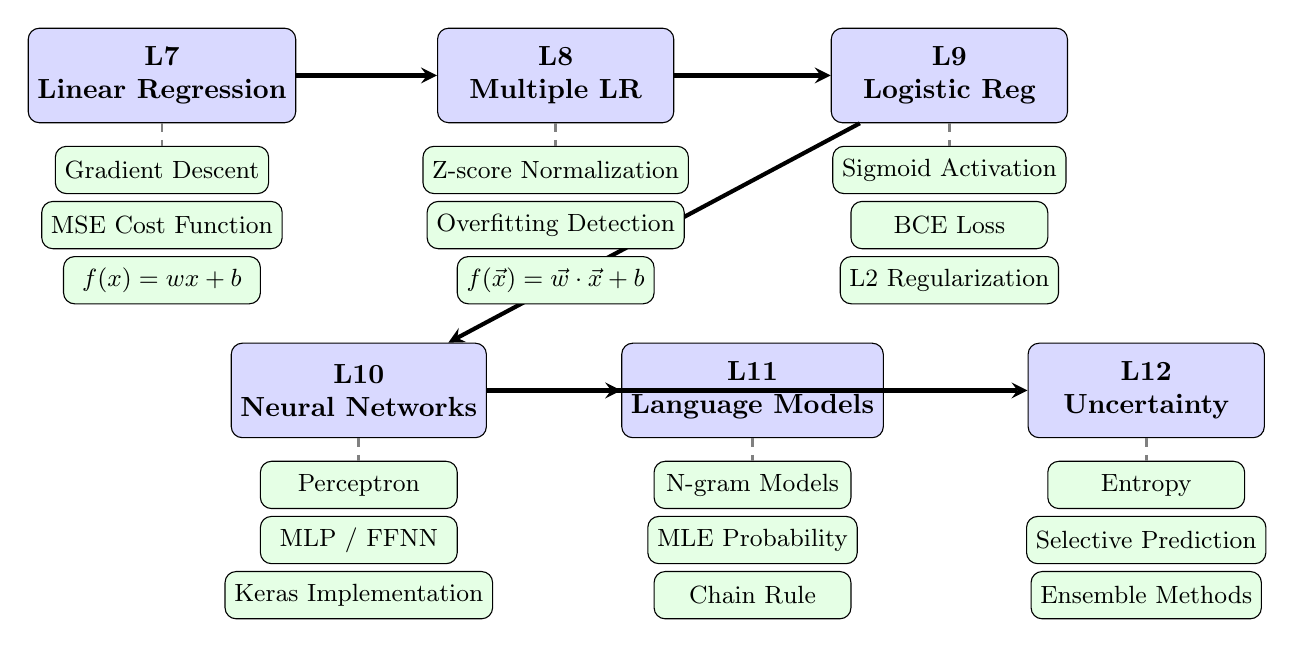
\begin{tikzpicture}[
    lec/.style={rectangle, draw, rounded corners, minimum width=3cm, minimum height=1.2cm, font=\normalsize\bfseries, fill=blue!15, align=center},
    concept/.style={rectangle, draw, rounded corners, minimum width=2.5cm, minimum height=0.6cm, font=\small, fill=green!10},
    arrow/.style={->, thick, >=stealth, line width=1.5pt}]

    % Row 1: Lectures L7-L9
    \node[lec] (l7) at (0,0) {L7\\Linear Regression};
    \node[lec] (l8) at (5,0) {L8\\Multiple LR};
    \node[lec] (l9) at (10,0) {L9\\Logistic Reg};

    % Row 2: Lectures L10-L12
    \node[lec] (l10) at (2.5,-4) {L10\\Neural Networks};
    \node[lec] (l11) at (7.5,-4) {L11\\Language Models};
    \node[lec] (l12) at (12.5,-4) {L12\\Uncertainty};

    % Connections
    \draw[arrow] (l7) -- (l8);
    \draw[arrow] (l8) -- (l9);
    \draw[arrow] (l9) -- (l10);
    \draw[arrow] (l10) -- (l11);
    \draw[arrow] (l10) -- (l12);

    % Concepts below L7
    \node[concept] (gd) at (0,-1.2) {Gradient Descent};
    \node[concept] (mse) at (0,-1.9) {MSE Cost Function};
    \node[concept] (model1) at (0,-2.6) {$f(x) = wx + b$};

    % Concepts below L8
    \node[concept] (zscore) at (5,-1.2) {Z-score Normalization};
    \node[concept] (overfit) at (5,-1.9) {Overfitting Detection};
    \node[concept] (multi) at (5,-2.6) {$f(\vec{x}) = \vec{w} \cdot \vec{x} + b$};

    % Concepts below L9
    \node[concept] (sigmoid) at (10,-1.2) {Sigmoid Activation};
    \node[concept] (bce) at (10,-1.9) {BCE Loss};
    \node[concept] (l2reg) at (10,-2.6) {L2 Regularization};

    % Concepts below L10
    \node[concept] (percep) at (2.5,-5.2) {Perceptron};
    \node[concept] (ffnn) at (2.5,-5.9) {MLP / FFNN};
    \node[concept] (keras) at (2.5,-6.6) {Keras Implementation};

    % Concepts below L11
    \node[concept] (ngram) at (7.5,-5.2) {N-gram Models};
    \node[concept] (mle) at (7.5,-5.9) {MLE Probability};
    \node[concept] (chain) at (7.5,-6.6) {Chain Rule};

    % Concepts below L12
    \node[concept] (entropy) at (12.5,-5.2) {Entropy};
    \node[concept] (selective) at (12.5,-5.9) {Selective Prediction};
    \node[concept] (ensemble) at (12.5,-6.6) {Ensemble Methods};

    % Vertical connectors
    \draw[dashed, gray, line width=1pt] (l7) -- (gd);
    \draw[dashed, gray, line width=1pt] (l8) -- (zscore);
    \draw[dashed, gray, line width=1pt] (l9) -- (sigmoid);
    \draw[dashed, gray, line width=1pt] (l10) -- (percep);
    \draw[dashed, gray, line width=1pt] (l11) -- (ngram);
    \draw[dashed, gray, line width=1pt] (l12) -- (entropy);
\end{tikzpicture}%
}
\end{center}

\begin{notebox}[The Red Thread]
\textbf{Regression} (L7-L8): Predict continuous values. Learn gradient descent, cost functions, normalization.

\textbf{Classification} (L9): Predict categories. Sigmoid activation, BCE loss, regularization.

\textbf{Neural Networks} (L10): Combine multiple units. Perceptron $\to$ MLP with hidden layers.

\textbf{Applications} (L11-L12): Language models use probability. Uncertainty measures confidence.
\end{notebox}

%% ========================================
%% KEY TERMS GLOSSARY
%% ========================================
\section{Key Terms Dictionary}

\begin{definitionbox}[Fundamental Concepts]

\textbf{Epoch}: One complete pass through ALL training examples. After 1 epoch, every sample has been seen once.

\textbf{Batch}: A subset of training data processed together. Batch size = number of samples per gradient update.

\textbf{Iteration}: One gradient update. If 1000 samples with batch size 100, then 10 iterations = 1 epoch.

\textbf{Learning Rate ($\alpha$)}: Step size for weight updates. Controls how much weights change per iteration.

\textbf{Gradient}: Direction of steepest increase in loss. We move opposite to gradient to minimize loss.

\textbf{Gradient Descent}: Algorithm that repeatedly updates weights: $w := w - \alpha \cdot \nabla J(w)$
\end{definitionbox}

\begin{definitionbox}[Model Types]

\textbf{Linear Regression}: $f(x) = wx + b$. Predicts continuous output. Uses MSE loss.

\textbf{Logistic Regression}: $f(x) = \sigma(wx + b)$. Binary classification. Uses BCE loss.

\textbf{Perceptron}: Single neuron. Binary output via threshold. Update: if wrong, adjust weights.

\textbf{MLP (Multi-Layer Perceptron)}: Neural network with hidden layers. Can learn non-linear boundaries.

\textbf{FFNN (Feed-Forward Neural Network)}: Same as MLP. Information flows forward only (no loops).

\textbf{CNN (Convolutional Neural Network)}: Specialized for images. Uses filters to detect patterns.
\end{definitionbox}

\begin{definitionbox}[Training Concepts]

\textbf{Training Set}: Data used to learn weights (typically 70-80\%).

\textbf{Validation Set}: Data used to tune hyperparameters and monitor overfitting (10-20\%).

\textbf{Test Set}: Data used ONCE for final evaluation. Never tune based on test results.

\textbf{Overfitting}: Model memorizes training data, fails on new data. Train acc high, val acc low.

\textbf{Underfitting}: Model too simple to capture patterns. Both train and val accuracy low.

\textbf{Regularization}: Technique to prevent overfitting. L2 adds penalty $\frac{\lambda}{2m}\sum w_j^2$ to cost.

\textbf{Oscillation}: When the loss goes up and down instead of steadily decreasing during training. Usually caused by a learning rate that is too high. Solution: reduce the learning rate.
\end{definitionbox}

\begin{definitionbox}[Activation Functions]

\textbf{Sigmoid}: $\sigma(z) = \frac{1}{1+e^{-z}}$. Output in $(0,1)$. Used for binary output.

\textbf{ReLU}: $\max(0, z)$. Output in $[0, \infty)$. Default for hidden layers.

\textbf{Softmax}: $\frac{e^{z_i}}{\sum_j e^{z_j}}$. Outputs sum to 1. Used for multi-class output.
\end{definitionbox}

\begin{definitionbox}[Loss Functions]

\textbf{MSE (Mean Squared Error)}: $\frac{1}{2m}\sum(f(x) - y)^2$. For regression.

\textbf{BCE (Binary Cross-Entropy)}: $-[y\log(\hat{y}) + (1-y)\log(1-\hat{y})]$. For binary classification.

\textbf{CE (Categorical Cross-Entropy)}: $-\sum_k y_k \log(\hat{y}_k)$. For multi-class classification.
\end{definitionbox}

\begin{definitionbox}[Uncertainty Concepts]

\textbf{Entropy}: $H = -\sum p_i \log_2(p_i)$. Measures uncertainty. $H=0$ means certain, $H=\log_2(K)$ means maximum uncertainty.

\textbf{Selective Prediction}: Only predict when confidence exceeds threshold. Trade accuracy for coverage.

\textbf{Ensemble}: Combine multiple models. Average their predictions to reduce variance.
\end{definitionbox}

%% ========================================
%% LECTURE 7: LINEAR REGRESSION
%% ========================================
\section{L7: Linear Regression}

\begin{definitionbox}[What You Learn]

\textbf{Goal}: Predict continuous values (e.g., house price from size).

\textbf{Model}: $f_{w,b}(x) = wx + b$ where $w$ = weight, $b$ = bias.

\textbf{Cost Function} (MSE):
\[J(w,b) = \frac{1}{2m}\sum_{i=1}^{m}(f_{w,b}(x^{(i)}) - y^{(i)})^2\]

\textbf{Why $\frac{1}{2m}$?} The $\frac{1}{2}$ makes gradient cleaner (cancels with derivative of square).
\end{definitionbox}

\begin{examplebox}[Gradient Descent Algorithm]

\textbf{Repeat until convergence}:
\begin{align*}
w &:= w - \alpha \frac{\partial J}{\partial w} = w - \alpha \cdot \frac{1}{m}\sum_{i=1}^{m}(f(x^{(i)}) - y^{(i)}) \cdot x^{(i)} \\
b &:= b - \alpha \frac{\partial J}{\partial b} = b - \alpha \cdot \frac{1}{m}\sum_{i=1}^{m}(f(x^{(i)}) - y^{(i)})
\end{align*}

\textbf{Key Insight}: Gradient points to steeper loss. Move opposite direction.
\end{examplebox}

\begin{notebox}[Key Takeaways L7]

\begin{itemize}[leftmargin=*,nosep]
\item Gradient descent finds optimal $w$, $b$ by minimizing cost
\item Learning rate $\alpha$ controls step size (too big = overshoot, too small = slow)
\item Cost should decrease each iteration (if not, check $\alpha$)
\item Single feature: one weight $w$
\end{itemize}
\end{notebox}

%% ========================================
%% LECTURE 8: MULTIPLE LINEAR REGRESSION
%% ========================================
\section{L8: Multiple Linear Regression}

\begin{definitionbox}[What You Learn]

\textbf{Goal}: Multiple features (e.g., house price from size, bedrooms, age, floors).

\textbf{Model}: $f_{\vec{w},b}(\vec{x}) = \vec{w} \cdot \vec{x} + b = w_1x_1 + w_2x_2 + ... + w_nx_n + b$

\textbf{Notation}: $\vec{x}^{(i)}$ = feature vector for example $i$, $x_j^{(i)}$ = feature $j$ of example $i$
\end{definitionbox}

\begin{warningbox}[Z-Score Normalization]

\textbf{Problem}: Features on different scales cause slow/unstable convergence.

\textbf{Solution}: Normalize each feature to mean=0, std=1:
\[x_{norm} = \frac{x - \mu}{\sigma}\]

\textbf{Critical Rules}:
\begin{enumerate}[leftmargin=*,nosep]
\item Compute $\mu$, $\sigma$ from TRAINING data only
\item Store $\mu$, $\sigma$ for later use
\item Apply SAME $\mu$, $\sigma$ to validation and test data
\end{enumerate}

\textbf{Never} compute $\mu$, $\sigma$ on test data (data leakage!)
\end{warningbox}

\begin{examplebox}[Overfitting Detection]

\textbf{Polynomial Features}: $x \to [x, x^2, x^3, ...]$ increases model complexity.

\textbf{Problem}: High-degree polynomials fit training data perfectly but fail on new data.

\textbf{Solution}: Monitor validation cost. If train cost keeps decreasing but val cost increases $\to$ overfitting!
\end{examplebox}

\begin{notebox}[Key Takeaways L8]

\begin{itemize}[leftmargin=*,nosep]
\item Multiple features use dot product: $\vec{w} \cdot \vec{x}$
\item ALWAYS normalize features before training
\item Split data: Train/Val/Test to detect overfitting
\item Simple models generalize better (Occam's Razor)
\end{itemize}
\end{notebox}

%% ========================================
%% LECTURE 9: LOGISTIC REGRESSION
%% ========================================
\section{L9: Logistic Regression}

\begin{definitionbox}[What You Learn]

\textbf{Goal}: Binary classification (e.g., spam/not spam, tumor malignant/benign).

\textbf{Model}: $f_{\vec{w},b}(\vec{x}) = \sigma(\vec{w} \cdot \vec{x} + b)$

\textbf{Sigmoid Function}:
\[\sigma(z) = \frac{1}{1 + e^{-z}}\]

\textbf{Properties}: Output always in $(0, 1)$. Interpret as probability $P(y=1|x)$.
\end{definitionbox}

\begin{warningbox}[Binary Cross-Entropy Loss]

\textbf{Why not MSE?} For classification, MSE creates non-convex cost with many local minima.

\textbf{BCE Loss}:
\[J = -\frac{1}{m}\sum_{i=1}^{m}[y^{(i)}\log(\hat{y}^{(i)}) + (1-y^{(i)})\log(1-\hat{y}^{(i)})]\]

\textbf{Intuition}:
\begin{itemize}[leftmargin=*,nosep]
\item If $y=1$: cost = $-\log(\hat{y})$ (penalize low predictions)
\item If $y=0$: cost = $-\log(1-\hat{y})$ (penalize high predictions)
\end{itemize}
\end{warningbox}

\begin{definitionbox}[L2 Regularization]

\textbf{Purpose}: Prevent overfitting by penalizing large weights.

\textbf{Regularized Cost}:
\[J_{reg} = J_{original} + \frac{\lambda}{2m}\sum_{j=1}^{n} w_j^2\]

\textbf{Regularized Gradient}:
\[\frac{\partial J}{\partial w_j} = \frac{\partial J_{orig}}{\partial w_j} + \frac{\lambda}{m}w_j\]

\textbf{Note}: Bias $b$ is NOT regularized (only weights $w_j$).

\textbf{$\lambda$ effect}: Larger $\lambda$ = smaller weights = simpler model = less overfitting (but risk underfitting).
\end{definitionbox}

\begin{examplebox}[Typical $\lambda$ Values and When to Use Them]
\begin{tabular}{@{}l|l|l@{}}
\textbf{$\lambda$ Value} & \textbf{When to Use} & \textbf{Effect on Model} \\
\hline
0 & No regularization needed & Weights can grow large \\
0.0001 & Very mild regularization & Almost no constraint \\
0.001 & Light regularization & Slight weight shrinkage \\
\textbf{0.01} & \textbf{Good starting point} & \textbf{Balanced constraint} \\
0.1 & Strong regularization & Significant weight shrinkage \\
1.0 & Very strong & Weights forced very small \\
10.0 & Extreme (rarely used) & Model becomes too simple \\
\end{tabular}

\vspace{0.5em}
\textbf{Keras syntax}: \texttt{kernel\_regularizer=regularizers.L2(0.01)}

\textbf{How to choose $\lambda$}:
\begin{enumerate}[leftmargin=*,nosep]
\item Start with $\lambda = 0.01$
\item If still overfitting (train acc $>>$ val acc): try $\lambda = 0.1$
\item If underfitting (both acc low): try $\lambda = 0.001$ or $\lambda = 0$
\item Common search: $[0.0001, 0.001, 0.01, 0.1, 1.0]$
\end{enumerate}
\end{examplebox}

\begin{notebox}[Key Takeaways L9]

\begin{itemize}[leftmargin=*,nosep]
\item Sigmoid squashes output to probability
\item Decision boundary: predict 1 if $f(x) \geq 0.5$
\item BCE loss is convex (guaranteed to find global minimum)
\item L2 regularization: use when overfitting (high train acc, low val acc)
\end{itemize}
\end{notebox}

%% ========================================
%% LECTURE 10: NEURAL NETWORKS
%% ========================================
\section{L10: Neural Networks}

\begin{definitionbox}[Perceptron]

\textbf{What}: Single artificial neuron. Simplest neural unit.

\textbf{Model}: $f(\vec{x}) = \text{step}(\vec{w} \cdot \vec{x} + b)$

\textbf{Decision}: Output 1 if $\vec{w} \cdot \vec{x} + b > 0$, else 0.

\textbf{Learning Rule}: If prediction wrong:
\begin{itemize}[leftmargin=*,nosep]
\item If should be 1 but predicted 0: $w := w + \alpha \cdot x$
\item If should be 0 but predicted 1: $w := w - \alpha \cdot x$
\end{itemize}

\textbf{Limitation}: Can only learn linearly separable patterns (fails on XOR).
\end{definitionbox}

\begin{definitionbox}[MLP / FFNN]

\textbf{Solution to Perceptron Limitation}: Stack multiple layers.

\textbf{Architecture}:
\begin{itemize}[leftmargin=*,nosep]
\item \textbf{Input layer}: Receives features (not counted as layer)
\item \textbf{Hidden layers}: Learn intermediate representations. Use ReLU activation.
\item \textbf{Output layer}: Produces final prediction. Sigmoid (binary) or Softmax (multi-class).
\end{itemize}

\textbf{Why ``Hidden''?} We don't directly observe their outputs during training.

\textbf{Universal Approximator}: MLP with 1+ hidden layer can approximate any continuous function.
\end{definitionbox}

\begin{examplebox}[Keras Pattern]

\begin{verbatim}
model = keras.Sequential([
    layers.Input(shape=(n_features,)),
    layers.Dense(64, activation="relu"),
    layers.Dense(32, activation="relu"),
    layers.Dense(1, activation="sigmoid")  # Binary
])
model.compile(
    optimizer=Adam(learning_rate=0.001),
    loss="binary_crossentropy",
    metrics=["accuracy"]
)
history = model.fit(X_train, y_train,
    validation_split=0.2,
    epochs=100, batch_size=32)
\end{verbatim}
\end{examplebox}

\begin{notebox}[Key Takeaways L10]

\begin{itemize}[leftmargin=*,nosep]
\item Perceptron: single neuron, linear boundary only
\item MLP: multiple layers enable non-linear boundaries
\item Hidden layers: ReLU activation (avoids vanishing gradient)
\item Output layer: Sigmoid (binary), Softmax (multi-class)
\item More layers/neurons = more capacity = more overfitting risk
\end{itemize}
\end{notebox}

%% ========================================
%% LECTURE 11: LANGUAGE MODELING
%% ========================================
\section{L11: Language Modeling}

\begin{definitionbox}[What You Learn]

\textbf{Goal}: Predict probability of word sequences.

\textbf{Application}: Auto-complete, spell-check, machine translation.

\textbf{Key Question}: Given context words, what's the probability of next word?
\end{definitionbox}

\begin{definitionbox}[N-gram Models]

\textbf{Idea}: Approximate probability using previous $n-1$ words.

\textbf{Bigram} ($n=2$): Condition on previous 1 word.
\[P(w_i | w_{i-1}) = \frac{C(w_{i-1}, w_i)}{C(w_{i-1})}\]

\textbf{Trigram} ($n=3$): Condition on previous 2 words.
\[P(w_i | w_{i-2}, w_{i-1}) = \frac{C(w_{i-2}, w_{i-1}, w_i)}{C(w_{i-2}, w_{i-1})}\]

\textbf{MLE} (Maximum Likelihood Estimation): Count occurrences, divide by context count.
\end{definitionbox}

\begin{examplebox}[Sentence Probability]

\textbf{Chain Rule}: $P(w_1, w_2, ..., w_n) = \prod_i P(w_i | w_1, ..., w_{i-1})$

\textbf{Bigram Approximation}:
\[P(\text{``the cat sat''}) = P(\text{the}) \cdot P(\text{cat}|\text{the}) \cdot P(\text{sat}|\text{cat})\]

\textbf{Example}: If $C(\text{the cat}) = 50$ and $C(\text{the}) = 1000$:
\[P(\text{cat}|\text{the}) = \frac{50}{1000} = 0.05\]
\end{examplebox}

\begin{notebox}[Key Takeaways L11]

\begin{itemize}[leftmargin=*,nosep]
\item N-gram: use last $n-1$ words to predict next
\item Bigger $n$ = more context = better but sparse counts
\item MLE = count-based probability estimation
\item Smoothing needed for unseen word combinations
\end{itemize}
\end{notebox}

%% ========================================
%% LECTURE 12: UNCERTAINTY
%% ========================================
\section{L12: Uncertainty}

\begin{definitionbox}[What You Learn]

\textbf{Goal}: Know when your model is uncertain about its predictions.

\textbf{Why Important?} High confidence wrong predictions are dangerous. Better to say ``I don't know.''
\end{definitionbox}

\begin{definitionbox}[Entropy as Uncertainty Measure]

\textbf{Formula}:
\[H = -\sum_{i=1}^{K} p_i \log_2(p_i)\]

\textbf{What are these $p_i$ values?} They are the softmax output probabilities. For a 2-class problem, the model outputs something like $[p_{\text{cat}}, p_{\text{dog}}]$ where both sum to 1.

\textbf{Interpretation}:
\begin{itemize}[leftmargin=*,nosep]
\item $H = 0$: Completely certain (one class has $p=1$, others have $p=0$)
\item $H = \log_2(K)$: Maximum uncertainty (all classes equally likely)
\item $2^H$: Effective number of classes the model is ``considering''
\end{itemize}
\end{definitionbox}

\begin{examplebox}[Understanding Softmax Output Probabilities]
\textbf{What does $[0.9, 0.1]$ mean?}

For a cat vs dog classifier:
\begin{itemize}[leftmargin=*,nosep]
\item $[0.9, 0.1]$ means: 90\% confident it's a cat, 10\% it's a dog
\item $[0.5, 0.5]$ means: 50\% cat, 50\% dog (model is guessing!)
\item $[0.99, 0.01]$ means: 99\% confident it's a cat (very sure)
\end{itemize}

\textbf{Entropy examples} (2 classes):  \newline
\begin{tabular}{@{}l|l|l@{}}
\textbf{Output Probabilities} & \textbf{Entropy $H$} & \textbf{Model is...} \\
\hline
$[1.0, 0.0]$ (100\% one class) & $H = 0$ & Completely certain \\
$[0.9, 0.1]$ (90\% vs 10\%) & $H \approx 0.47$ & Quite confident \\
$[0.7, 0.3]$ (70\% vs 30\%) & $H \approx 0.88$ & Somewhat uncertain \\
$[0.5, 0.5]$ (50\% vs 50\%) & $H = 1.0$ & Maximum uncertainty \\
\end{tabular}

\textbf{Rule}: Lower entropy = more confident. Higher entropy = more uncertain.
\end{examplebox}

\begin{examplebox}[Selective Prediction with Confidence Threshold]

\textbf{Idea}: Only predict when the model's highest probability exceeds a threshold.

\textbf{Confidence} = the maximum probability in the output = $\max(p_1, p_2, ..., p_K)$

\textbf{Example}: If output is $[0.7, 0.2, 0.1]$ for 3 classes, confidence = 0.7 (70\%)

\begin{tabular}{@{}l|l|l|l@{}}
\textbf{Threshold} & \textbf{Meaning} & \textbf{Result} & \textbf{Trade-off} \\
\hline
0.5 (50\%) & Predict if $>$50\% sure & More predictions & Lower accuracy \\
0.7 (70\%) & Predict if $>$70\% sure & Medium & Balanced \\
0.9 (90\%) & Predict if $>$90\% sure & Fewer predictions & Higher accuracy \\
\end{tabular}

\textbf{With threshold = 0.8}:
\begin{itemize}[leftmargin=*,nosep]
\item Output $[0.85, 0.15]$: Confidence = 0.85 $\geq$ 0.8, so PREDICT class 0
\item Output $[0.6, 0.4]$: Confidence = 0.6 $<$ 0.8, so ABSTAIN (don't predict)
\end{itemize}
\end{examplebox}

\begin{definitionbox}[Ensemble Methods]

\textbf{Idea}: Train multiple models, average their predictions.

\textbf{Formula}:
\[P_{ensemble}(c) = \frac{1}{N}\sum_{i=1}^{N} P_{model_i}(c)\]

\textbf{Benefits}:
\begin{itemize}[leftmargin=*,nosep]
\item Reduces variance (less overfitting)
\item Better uncertainty estimates
\item Models disagree on hard/ambiguous examples
\end{itemize}

\textbf{Disagreement = Uncertainty}: If models give different predictions, the example is likely hard.
\end{definitionbox}

\begin{notebox}[Key Takeaways L12]

\begin{itemize}[leftmargin=*,nosep]
\item Entropy quantifies prediction uncertainty
\item Low entropy = confident, high entropy = uncertain
\item Selective prediction: trade coverage for accuracy
\item Ensembles: average models for better predictions and uncertainty
\end{itemize}
\end{notebox}

%% ========================================
%% QUICK LOOKUP TABLES
%% ========================================
\section{Quick Lookup Tables}

\begin{definitionbox}[Task to Model Mapping]

\begin{tabular}{@{}l|l|l|l@{}}
\textbf{Task} & \textbf{Model} & \textbf{Output} & \textbf{Loss} \\
\hline
Predict price & Linear Reg & Linear & MSE \\
Yes/No & Logistic Reg & Sigmoid(1) & BCE \\
Multi-class & MLP & Softmax(K) & CE \\
Next word & N-gram & Probability & Log-loss \\
\end{tabular}
\end{definitionbox}

\begin{definitionbox}[Problem to Solution Mapping]

\begin{tabular}{@{}l|l@{}}
\textbf{Problem} & \textbf{Solution} \\
\hline
Features on different scales & Z-score normalization \\
Model overfitting & L2 regularization, more data, simpler model \\
Model underfitting & More neurons/layers, less regularization \\
Slow convergence & Check learning rate, normalize features \\
Loss oscillating & Decrease learning rate \\
Loss stuck high & Increase learning rate or model capacity \\
Want confidence info & Use entropy, selective prediction \\
Want better accuracy & Use ensemble of models \\
\end{tabular}
\end{definitionbox}

\begin{definitionbox}[Formula Quick Reference]

\textbf{Gradient Descent} \hfill $w := w - \alpha \frac{\partial J}{\partial w}$ \\
\textit{Update weight by stepping opposite to gradient, scaled by learning rate.}

\textbf{Sigmoid} \hfill $\sigma(z) = \frac{1}{1 + e^{-z}}$ \\
\textit{Squashes any input to a value between 0 and 1 (probability).}

\textbf{Softmax} \hfill $\frac{e^{z_i}}{\sum_j e^{z_j}}$ \\
\textit{Converts scores to probabilities that sum to 1 across all classes.}

\textbf{MSE} \hfill $\frac{1}{2m}\sum(f(x) - y)^2$ \\
\textit{Average squared difference between prediction and actual value.}

\textbf{BCE} \hfill $-[y\log\hat{y} + (1-y)\log(1-\hat{y})]$ \\
\textit{Penalizes confident wrong predictions heavily (binary classification).}

\textbf{L2 Cost} \hfill $J + \frac{\lambda}{2m}\sum w_j^2$ \\
\textit{Original cost plus penalty for large weights (prevents overfitting).}

\textbf{Z-score} \hfill $\frac{x - \mu}{\sigma}$ \\
\textit{Center data at 0, scale to unit variance (normalize features).}

\textbf{Entropy} \hfill $-\sum p_i \log_2(p_i)$ \\
\textit{Measures uncertainty: 0 = certain, higher = more uncertain.}

\textbf{Bigram} \hfill $\frac{C(w_{i-1}, w_i)}{C(w_{i-1})}$ \\
\textit{Probability of word given previous word (count-based).}
\end{definitionbox}

\begin{examplebox}[Lecture to Keras Component]

\begin{tabular}{@{}l|l@{}}
\textbf{Concept} & \textbf{Keras Code} \\
\hline
Hidden layer & \texttt{Dense(64, activation='relu')} \\
Binary output & \texttt{Dense(1, activation='sigmoid')} \\
Multi-class output & \texttt{Dense(K, activation='softmax')} \\
L2 regularization & \texttt{kernel\_regularizer=regularizers.L2(0.01)} \\
Binary loss & \texttt{loss='binary\_crossentropy'} \\
Multi-class loss & \texttt{loss='sparse\_categorical\_crossentropy'} \\
Optimizer & \texttt{optimizer=Adam(learning\_rate=0.001)} \\
Validation & \texttt{validation\_split=0.2} \\
\end{tabular}
\end{examplebox}

%% ########################################
%% PAGE BREAK - PART B STARTS ON NEW PAGE
%% ########################################
\newpage

%% ########################################
%% PART B: TRAINING GUIDE (ORIGINAL CONTENT)
%% ########################################

\begin{center}
\textbf{\LARGE PART B: Training Guide \& Reference Tables}
\end{center}
\vspace{1em}

%% ========================================
%% SECTION 0: FEATURE INSIGHTS (DATA ANALYSIS)
%% ========================================
\renewcommand{\thesection}{B.\arabic{section}}
\setcounter{section}{9}
\section{Feature Insights at a Glance}

\begin{definitionbox}[Reading Bar Charts for Feature Importance]

\textbf{Goal}: Quickly identify which features help predict the target.

\textbf{Method}: Plot feature vs target mean. Look at bar heights.

\textbf{Informative Feature}: Bars have DIFFERENT heights across categories.
\begin{itemize}[leftmargin=*,nosep]
\item Example: ``education'' shows high school avg=40K, bachelor's avg=65K, master's avg=85K
\item Clear difference = feature helps distinguish outcomes
\end{itemize}

\textbf{Non-Informative Feature}: Bars have SIMILAR heights across categories.
\begin{itemize}[leftmargin=*,nosep]
\item Example: ``eye color'' shows blue avg=52K, brown avg=51K, green avg=53K
\item Almost same = feature doesn't help much
\end{itemize}
\end{definitionbox}

\begin{examplebox}[Visual Pattern Recognition]

\begin{tabular}{@{}l|l|l@{}}
\textbf{What You See} & \textbf{Meaning} & \textbf{Action} \\
\hline
Big height differences & Strong predictor & Keep feature \\
Small height differences & Weak predictor & Consider dropping \\
Clear trend (up/down) & Linear relationship & Good for model \\
Random/no pattern & No relationship & May add noise \\
One bar much higher & Category matters & Keep feature \\
All bars same height & No discrimination & Less useful \\
\end{tabular}
\end{examplebox}

\begin{warningbox}[Quick Feature Selection Rules]

\textbf{MOST Informative} (keep these):
\begin{itemize}[leftmargin=*,nosep]
\item Features where target mean varies a lot between categories
\item Features showing clear trends (monotonic increase/decrease)
\item Features with distinct separation between groups
\end{itemize}

\textbf{LEAST Informative} (consider removing):
\begin{itemize}[leftmargin=*,nosep]
\item Features where all categories have similar target mean
\item Features with high variance but no clear pattern
\item Features with too many missing values
\end{itemize}

\end{warningbox}

\begin{notebox}[Numeric vs Categorical Features]

\textbf{Categorical} (discrete values): Use bar charts, count plots.

\textbf{Numeric} (continuous values): Use scatter plots, correlation.

\textbf{Tip}: Bar charts make it easy to compare category means at a glance.
\end{notebox}

%% ========================================
%% SECTION 1: TRAINING FUNDAMENTALS
%% ========================================
\section{Training Fundamentals}

\begin{definitionbox}[Core Terminology]

\textbf{Epoch}: One complete pass through all training data.

\textbf{Batch Size}: Number of samples per gradient update.

\textbf{Learning Rate ($\alpha$)}: Step size for weight updates.

\textbf{Validation Split}: Fraction held out for monitoring.

\textbf{Gradient}: Direction of steepest loss increase.

\textbf{Loss/Cost ($J$)}: Measures prediction error.
\end{definitionbox}

\begin{definitionbox}[When You INCREASE Each Parameter]

\begin{tabular}{@{}l|l|l@{}}
\textbf{Increase...} & \textbf{What Happens} & \textbf{Risk} \\
\hline
Learning Rate & Faster training & Divergence \\
Batch Size & Faster per epoch & Worse generalization \\
Epochs & More learning & Overfitting \\
Regularization ($\lambda$) & Smaller weights & Underfitting \\
Hidden Neurons & Higher capacity & Overfitting \\
Hidden Layers & More abstraction & Harder to train \\
\end{tabular}
\end{definitionbox}

\begin{examplebox}[Hyperparameter Starting Values]

\begin{tabular}{@{}l|c|c|c@{}}
\textbf{Parameter} & \textbf{Start} & \textbf{Range} & \textbf{Adjust If...} \\
\hline
Learning Rate & 0.001 & 0.0001--0.1 & Oscillating/slow \\
Batch Size & 32 & 16--256 & Memory/speed \\
Epochs & 100 & 50--500 & Under/overfit \\
Val Split & 0.2 & 0.1--0.3 & Dataset size \\
L2 $\lambda$ & 0.01 & 0.001--0.1 & Overfitting \\
Hidden Neurons & 64 & 32--256 & Capacity \\
Hidden Layers & 1 & 1--3 & Complexity \\
\end{tabular}
\end{examplebox}

%% ========================================
%% DATASET SIZE CONFIGURATIONS
%% ========================================
\subsection*{Dataset Size $\to$ Hyperparameter Configuration}

\begin{warningbox}[Binary Classification by Dataset Size]

\resizebox{\linewidth}{!}{%
\begin{tabular}{@{}l|cccc@{}}
\textbf{Parameter} & \textbf{Small ($<$1K)} & \textbf{Med (1K-10K)} & \textbf{Large (10K-100K)} & \textbf{V.Large ($>$100K)} \\
\hline
Learning Rate & 0.001 & 0.001 & 0.001--0.01 & 0.01 \\
Batch Size & 16 & 32 & 64--128 & 128--256 \\
Epochs & 50--100 & 100--200 & 50--100 & 20--50 \\
Val Split & 0.3 & 0.2 & 0.15 & 0.1 \\
L2 $\lambda$ & 0.1 & 0.01 & 0.001--0.01 & 0.001 \\
Hidden Neurons & 16--32 & 32--64 & 64--128 & 128--256 \\
Hidden Layers & 1 & 1--2 & 2 & 2--3 \\
\end{tabular}}

\vspace{0.5em}
\textbf{Key insights}:
\begin{itemize}[leftmargin=*,nosep]
\item Small data $\to$ high $\lambda$ (0.1), few neurons, large val split (30\%)
\item More data $\to$ can reduce regularization, add capacity
\item Large batch = faster training but may generalize worse
\item Fewer epochs needed when dataset is large (sees more per epoch)
\item Always start simple, add complexity only if underfitting
\end{itemize}
\end{warningbox}

\begin{warningbox}[MLP (Multi-Class) by Dataset Size]

\resizebox{\linewidth}{!}{%
\begin{tabular}{@{}l|cccc@{}}
\textbf{Parameter} & \textbf{Small ($<$1K)} & \textbf{Med (1K-10K)} & \textbf{Large (10K-100K)} & \textbf{V.Large ($>$100K)} \\
\hline
Learning Rate & 0.0001--0.001 & 0.001 & 0.001 & 0.001--0.01 \\
Batch Size & 16 & 32 & 64--128 & 256 \\
Epochs & 100--200 & 100--150 & 50--100 & 10--30 \\
Val Split & 0.3 & 0.2 & 0.15 & 0.05--0.1 \\
L2 $\lambda$ & 0.1--0.5 & 0.01--0.1 & 0.001--0.01 & 0.0001--0.001 \\
Hidden Neurons & 32 & 64--128 & 128--256 & 256--512 \\
Hidden Layers & 1 & 1--2 & 2--3 & 3+ \\
Output Activ. & softmax & softmax & softmax & softmax \\
\end{tabular}}

\vspace{0.5em}
\textbf{Key insights}:
\begin{itemize}[leftmargin=*,nosep]
\item Multi-class needs lower LR than binary (more complex optimization)
\item Small data + many classes = very high overfit risk $\to$ strong $\lambda$
\item Large data allows 3+ layers and 256+ neurons per layer
\item Softmax output always for multi-class (probabilities sum to 1)
\item With $>$100K samples, can use aggressive batch sizes (256) for speed
\end{itemize}
\end{warningbox}

\begin{warningbox}[Linear Regression by Dataset Size]

\resizebox{\linewidth}{!}{%
\begin{tabular}{@{}l|cccc@{}}
\textbf{Parameter} & \textbf{Small ($<$1K)} & \textbf{Med (1K-10K)} & \textbf{Large (10K-100K)} & \textbf{V.Large ($>$100K)} \\
\hline
Learning Rate & 0.001 & 0.001--0.01 & 0.01 & 0.01--0.1 \\
Batch Size & 16 & 32 & 64--128 & 128--256 \\
Epochs & 100--200 & 100--150 & 50--100 & 20--50 \\
Val Split & 0.3 & 0.2 & 0.15 & 0.1 \\
L2 $\lambda$ & 0.01--0.1 & 0.001--0.01 & 0.001 & 0.0001--0.001 \\
Hidden Neurons & 16--32 & 32--64 & 64--128 & 128--256 \\
Hidden Layers & 1 & 1--2 & 2 & 2--3 \\
Output Activ. & linear & linear & linear & linear \\
Loss Function & mse & mse & mse & mse \\
\end{tabular}}

\vspace{0.5em}
\textbf{Key insights}:
\begin{itemize}[leftmargin=*,nosep]
\item Regression tolerates higher LR than classification (simpler loss surface)
\item Output is always \texttt{linear} (no activation) for unbounded predictions
\item MSE loss standard; use MAE if many outliers
\item Small data $\to$ regularization prevents overfitting to noise
\item Larger batch sizes OK for regression (less noisy gradients needed)
\end{itemize}
\end{warningbox}

\begin{notebox}[Dataset Size Rules of Thumb]

\textbf{Small data ($<$1K samples)}:
\begin{itemize}[leftmargin=*,nosep]
\item High overfitting risk $\to$ strong regularization ($\lambda = 0.1$)
\item Keep model simple (1 hidden layer, few neurons)
\item Use larger validation split (30\%) for reliable estimates
\item Consider simpler models (Logistic Regression) first
\end{itemize}

\textbf{Medium data (1K--10K samples)}:
\begin{itemize}[leftmargin=*,nosep]
\item Balanced approach: moderate regularization ($\lambda = 0.01$)
\item Can use 1--2 hidden layers with 64 neurons
\item Standard validation split (20\%)
\end{itemize}

\textbf{Large data ($>$10K samples)}:
\begin{itemize}[leftmargin=*,nosep]
\item Lower overfitting risk $\to$ less regularization needed
\item Can use deeper networks (2--3 layers, 128+ neurons)
\item Smaller validation split OK (10--15\%)
\item Larger batch sizes for faster training
\end{itemize}
\end{notebox}

%% ========================================
%% SECTION 2: TRAINING CURVES INTERPRETATION
%% ========================================
\section{Training Curve Patterns}

\begin{warningbox}[Loss Curve Diagnosis]

\begin{tabular}{@{}l|l|l@{}}
\textbf{You See...} & \textbf{Problem} & \textbf{Fix} \\
\hline
Both losses decrease & Good! & Keep going \\
Train decreases, Val increases & Overfitting & Add regularization \\
Both stuck high & Underfitting & Increase model size \\
Wild oscillation & LR too high & Divide LR by 10 \\
Very slow decrease & LR too low & Multiply LR by 10 \\
Loss becomes NaN & Exploding gradient & Lower LR, check data \\
\end{tabular}
\end{warningbox}

\begin{definitionbox}[Accuracy-Based Diagnosis]

\begin{tabular}{@{}cc|l|l@{}}
\textbf{Train} & \textbf{Val} & \textbf{Status} & \textbf{Fix} \\
\hline
Low & Low & Underfitting & Bigger model, less $\lambda$, more epochs \\
High & Low & Overfitting & More $\lambda$, smaller model, more data \\
High & High & Good fit & Ready for test set \\
Low & High & Bug & Check your code/data \\
\end{tabular}
\end{definitionbox}

\begin{notebox}[Convergence Indicators]

\textbf{Converged}: Loss stops decreasing, train and val accuracy are similar.

\textbf{Not converged}: Loss is still going down noticeably.

\textbf{Early stopping}: Stop when validation loss stops improving.

\textbf{Patience}: Number of epochs to wait before stopping (typically 5-20).
\end{notebox}

%% ========================================
%% SECTION 3: LINEAR REGRESSION TRAINING
%% ========================================
\section{Linear Regression Training}

\begin{definitionbox}[Model Setup]

\textbf{Model}: $f(\vec{x}) = \vec{w} \cdot \vec{x} + b$

\textbf{Loss}: Mean Squared Error (MSE)
\[J = \frac{1}{2m}\sum_{i=1}^{m}(f(\vec{x}^{(i)}) - y^{(i)})^2\]

\textbf{Output}: 1 neuron + linear activation (no activation)

\textbf{Prediction}: Direct output value (no threshold needed)
\end{definitionbox}

\begin{examplebox}[Linear Regression Architecture]

\begin{center}
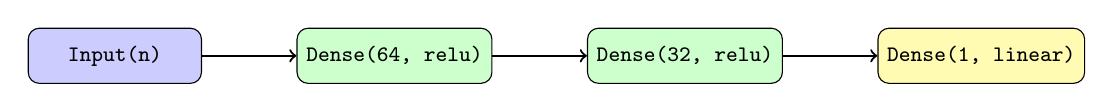
\begin{tikzpicture}[
    node distance=1.2cm,
    layer/.style={rectangle, draw, rounded corners, minimum width=2.2cm, minimum height=0.7cm, font=\footnotesize\ttfamily}]
    \node[layer, fill=blue!20] (input) {Input(n)};
    \node[layer, fill=green!20, right=of input] (hidden1) {Dense(64, relu)};
    \node[layer, fill=green!20, right=of hidden1] (hidden2) {Dense(32, relu)};
    \node[layer, fill=yellow!30, right=of hidden2] (output) {Dense(1, linear)};
    \draw[->, thick] (input) -- (hidden1);
    \draw[->, thick] (hidden1) -- (hidden2);
    \draw[->, thick] (hidden2) -- (output);
\end{tikzpicture}
\end{center}
\vspace{-0.5em}
\textbf{Compile}: \texttt{loss='mse', optimizer=Adam(lr=0.001), metrics=['mae']}
\end{examplebox}

\begin{definitionbox}[Linear Regression Parameters]

\begin{tabular}{@{}l|c|l@{}}
\textbf{Component} & \textbf{Value} & \textbf{Reason} \\
\hline
Output neurons & 1 & Single continuous value \\
Output activation & linear & Unbounded output range \\
Loss function & MSE & Penalizes squared error \\
Alternative loss & MAE & Robust to outliers \\
Metrics & mae & Interpretable error unit \\
\end{tabular}
\end{definitionbox}

\begin{notebox}[When to Use MAE vs MSE]

\textbf{MSE} (Mean Squared Error): Default choice. Penalizes large errors more heavily.
\begin{itemize}[leftmargin=*,nosep]
\item Use when: Large errors are especially bad
\item Sensitive to outliers (squares blow up)
\end{itemize}

\textbf{MAE} (Mean Absolute Error): More robust alternative.
\begin{itemize}[leftmargin=*,nosep]
\item Use when: Data has outliers you can't remove
\item Treats all errors equally (no squaring)
\end{itemize}

\textbf{Rule}: Start with MSE. If results are bad and you have outliers, try MAE.
\end{notebox}

%% ========================================
%% SECTION 4: BINARY CLASSIFICATION TRAINING
%% ========================================
\section{Binary Classification Training}

\begin{definitionbox}[Model Setup]

\textbf{Model}: $f(\vec{x}) = \sigma(\vec{w} \cdot \vec{x} + b)$

\textbf{Loss}: Binary Cross-Entropy (BCE)
\[L = -\frac{1}{m}\sum_{i=1}^{m}[y^{(i)}\log(\hat{y}^{(i)}) + (1-y^{(i)})\log(1-\hat{y}^{(i)})]\]

\textbf{Output}: 1 neuron + sigmoid activation

\textbf{Decision}: Predict 1 if $f(\vec{x}) \geq 0.5$, else 0
\end{definitionbox}

\begin{examplebox}[Binary Classification Architecture]

\begin{center}
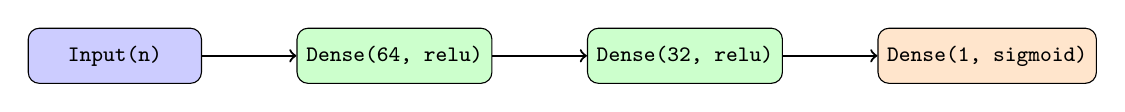
\begin{tikzpicture}[
    node distance=1.2cm,
    layer/.style={rectangle, draw, rounded corners, minimum width=2.2cm, minimum height=0.7cm, font=\footnotesize\ttfamily}]
    \node[layer, fill=blue!20] (input) {Input(n)};
    \node[layer, fill=green!20, right=of input] (hidden1) {Dense(64, relu)};
    \node[layer, fill=green!20, right=of hidden1] (hidden2) {Dense(32, relu)};
    \node[layer, fill=orange!20, right=of hidden2] (output) {Dense(1, sigmoid)};
    \draw[->, thick] (input) -- (hidden1);
    \draw[->, thick] (hidden1) -- (hidden2);
    \draw[->, thick] (hidden2) -- (output);
\end{tikzpicture}
\end{center}
\vspace{-0.5em}
\textbf{Compile}: \texttt{loss='binary\_crossentropy', optimizer=Adam(lr=0.001)}
\end{examplebox}

\begin{definitionbox}[Binary Classification Parameters]

\begin{tabular}{@{}l|c|l@{}}
\textbf{Component} & \textbf{Value} & \textbf{Reason} \\
\hline
Output neurons & 1 & Binary output \\
Output activation & sigmoid & Maps to $[0,1]$ \\
Loss function & BCE & Penalizes wrong conf. \\
Threshold & 0.5 & Decision boundary \\
Metrics & accuracy & Primary metric \\
\end{tabular}
\end{definitionbox}

%% ========================================
%% SECTION 4: MULTI-CLASS CLASSIFICATION
%% ========================================
\section{Multi-Class Classification}

\begin{definitionbox}[Model Setup]

\textbf{Output}: $K$ neurons + softmax activation

\textbf{Softmax}: $\text{softmax}(z_i) = \frac{e^{z_i}}{\sum_{j=1}^{K} e^{z_j}}$

\textbf{Loss}: Categorical Cross-Entropy
\[L = -\sum_{i=1}^{K} y_i \log(\hat{y}_i)\]

\textbf{Sparse vs Dense Labels}:
\begin{itemize}[leftmargin=*,nosep]
\item Integer labels (0,1,2,...): \texttt{sparse\_categorical\_crossentropy}
\item One-hot labels: \texttt{categorical\_crossentropy}
\end{itemize}
\end{definitionbox}

\begin{examplebox}[Multi-Class Architecture]

\begin{center}
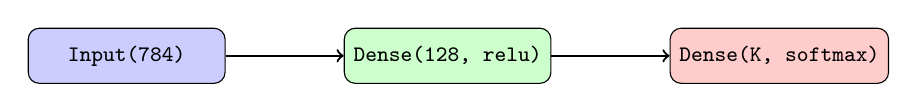
\begin{tikzpicture}[
    node distance=1.5cm,
    layer/.style={rectangle, draw, rounded corners, minimum width=2.5cm, minimum height=0.7cm, font=\footnotesize\ttfamily}]
    \node[layer, fill=blue!20] (input) {Input(784)};
    \node[layer, fill=green!20, right=of input] (hidden) {Dense(128, relu)};
    \node[layer, fill=red!20, right=of hidden] (output) {Dense(K, softmax)};
    \draw[->, thick] (input) -- (hidden);
    \draw[->, thick] (hidden) -- (output);
\end{tikzpicture}
\end{center}
\vspace{-0.5em}
\textbf{Compile}: \texttt{loss='sparse\_categorical\_crossentropy'}
\end{examplebox}

\begin{definitionbox}[Multi-Class Parameters]

\begin{tabular}{@{}l|c|l@{}}
\textbf{Component} & \textbf{Value} & \textbf{Reason} \\
\hline
Output neurons & $K$ (classes) & One per class \\
Output activation & softmax & Prob. distribution \\
Loss function & CE & Multi-class \\
Prediction & argmax & Highest prob. class \\
\end{tabular}
\end{definitionbox}

%% ========================================
%% SECTION 5: MLP ARCHITECTURE DESIGN
%% ========================================
\section{MLP Architecture Design}

\begin{definitionbox}[Architecture Decision Matrix]

\begin{tabular}{@{}l|l|l@{}}
\textbf{Decision} & \textbf{Options} & \textbf{Trade-off} \\
\hline
Hidden layers & 1--3 & Abstraction vs training \\
Neurons/layer & 32--256 & Capacity vs overfit \\
Hidden activation & ReLU & Default choice \\
Output activation & sigmoid/softmax & Task-dependent \\
Regularization & L2, Dropout & Overfit prevention \\
\end{tabular}
\end{definitionbox}

\begin{notebox}[Layer Design Guidelines]

\textbf{Width} (neurons per layer): More neurons = higher capacity but more overfitting risk.

\textbf{Depth} (number of layers): More layers = more abstract features but harder to train.

\textbf{Starting point}: 1-2 hidden layers, 64-128 neurons each.

\textbf{Common Patterns}:
\begin{itemize}[leftmargin=*,nosep]
\item Funnel: 128, then 64, then 32, then output
\item Constant: 64, then 64, then output
\item Pyramid (rare): 32, then 64, then output
\end{itemize}
\end{notebox}

\begin{examplebox}[Model Size vs Performance]

\begin{tabular}{@{}l|l|l|l@{}}
\textbf{Architecture} & \textbf{Params} & \textbf{Train Acc} & \textbf{Val Acc} \\
\hline
Dense(16) & ~160 & Medium & Medium \\
Dense(64) & ~650 & High & High (good) \\
Dense(256) & ~2500 & Very High & Lower (overfit) \\
Dense(64,64) & ~4500 & Very High & Low (overfit) \\
\end{tabular}

\textbf{Rule}: More parameters needs more data OR more regularization.
\end{examplebox}

%% ========================================
%% SECTION 6: REGULARIZATION
%% ========================================
\section{Regularization Techniques}

\begin{definitionbox}[L2 Regularization (Weight Decay)]

\textbf{Modified Cost}:
\[J_{reg} = J_{original} + \frac{\lambda}{2m}\sum_{j=1}^{n} w_j^2\]

\textbf{Modified Gradient}:
\[\frac{\partial J}{\partial w_j} = \frac{\partial J_{orig}}{\partial w_j} + \frac{\lambda}{m}w_j\]

\textbf{Effect}: Shrinks weights toward zero.

\textbf{Note}: Bias $b$ is NOT regularized.
\end{definitionbox}

\begin{examplebox}[$\lambda$ Effect on Training]

\begin{tabular}{@{}l|l|l|l@{}}
\textbf{$\lambda$ Value} & \textbf{Weights} & \textbf{Train Acc} & \textbf{Val Acc} \\
\hline
0 (none) & Large & High & Low (overfit) \\
0.001 (small) & Medium & High & Medium \\
0.01 (good start) & Moderate & Medium-High & High \\
0.1 (too high) & Very small & Low & Low (underfit) \\
\end{tabular}

\textbf{Goal}: Find $\lambda$ where Validation Accuracy is highest.
\end{examplebox}

\begin{warningbox}[Regularization Diagnosis]

\textbf{$\lambda$ too low}: Train accuracy much better than Val accuracy.

\textbf{Solution}: Increase $\lambda$ to reduce overfitting.

\textbf{$\lambda$ too high}: Both accuracies are low.

\textbf{Solution}: Decrease $\lambda$ to allow more learning.

\textbf{Just right}: Train and Val accuracy are close, both high.
\end{warningbox}

%% ========================================
%% SECTION 7: LEARNING RATE EFFECTS
%% ========================================
\section{Learning Rate Analysis}

\begin{definitionbox}[Learning Rate Behavior]

\begin{tabular}{@{}l|l|l@{}}
\textbf{LR Value} & \textbf{Loss Curve Looks Like} & \textbf{What To Do} \\
\hline
0.1+ (too high) & Oscillates or explodes & Divide by 10 \\
0.01 (high) & Fast but unstable & Monitor closely \\
0.001 (good) & Smooth decrease & Keep this value \\
0.0001 (low) & Very slow decrease & Multiply by 10 \\
1e-5 (too low) & Almost flat/no change & Multiply by 100 \\
\end{tabular}
\end{definitionbox}

\begin{notebox}[LR Interactions with Other Parameters]

\textbf{LR + Batch Size}: If you double batch size, often need to double LR too.

\textbf{LR + Epochs}: Lower LR needs more epochs to converge. Higher LR needs fewer epochs but is unstable.

\textbf{LR + Regularization}: Strong regularization ($\lambda$) slows learning. May need more epochs when $\lambda$ is high.
\end{notebox}

%% ========================================
%% SECTION 8: VALIDATION SPLIT
%% ========================================
\section{Validation \& Data Splitting}

\begin{definitionbox}[Data Split Strategy]

\begin{tabular}{@{}l|c|l@{}}
\textbf{Dataset Size} & \textbf{Val Split} & \textbf{Reasoning} \\
\hline
Small ($<$1K) & 0.3 & Need reliable val estimate \\
Medium (1K-10K) & 0.2 & Balance train/val \\
Large ($>$10K) & 0.1-0.15 & More data for training \\
Very Large ($>$100K) & 0.05-0.1 & Enough for both \\
\end{tabular}
\end{definitionbox}

\begin{notebox}[Three-Way Split]

\textbf{Training}: Used for learning weights (60-80\%)

\textbf{Validation}: Used for tuning hyperparameters (10-20\%)

\textbf{Test}: Used ONCE for final evaluation (10-20\%)

\textbf{Golden Rule}: NEVER tune based on test performance!
\end{notebox}

%% ========================================
%% SECTION 9: EPOCHS AND EARLY STOPPING
%% ========================================
\section{Epochs \& Early Stopping}

\begin{definitionbox}[Epoch Effects]

\begin{tabular}{@{}c|cc|l@{}}
\textbf{Epochs} & \textbf{Train Loss} & \textbf{Val Loss} & \textbf{Status} \\
\hline
10 & High & High & Underfit \\
50 & Medium & Medium & Learning \\
100 & Low & Low & Good fit \\
200 & Very Low & Rising & Overfit! \\
\end{tabular}
\end{definitionbox}

\begin{warningbox}[Early Stopping Protocol]

\textbf{Monitor}: Validation loss (not training loss)

\textbf{Patience}: Number of epochs without improvement

\textbf{Best model}: Save weights when val loss is lowest

\textbf{Typical patience}: 5-20 epochs

\textbf{Stop when}: Val loss hasn't improved for \texttt{patience} epochs
\end{warningbox}

%% ========================================
%% SECTION 10: FEATURE PREPROCESSING
%% ========================================
\section{Feature Preprocessing}

\begin{definitionbox}[Z-Score Normalization]

\textbf{Formula}: $x_{norm} = \frac{x - \mu}{\sigma}$

\textbf{Result}: Mean=0, Std=1

\textbf{Implementation}:
\begin{enumerate}[leftmargin=*,nosep]
\item Compute $\mu$, $\sigma$ from \textbf{training data only}
\item Store $\mu$, $\sigma$ for later use
\item Apply to train, val, and test data
\end{enumerate}
\end{definitionbox}

\begin{examplebox}[Normalization Impact]

\begin{tabular}{@{}l|cc@{}}
\textbf{Setting} & \textbf{Convergence} & \textbf{LR Needed} \\
\hline
No normalization & Slow/fails & Very small \\
With normalization & Fast & Standard (0.001) \\
\end{tabular}

\textbf{Why?} Features on different scales cause gradient descent to oscillate.
\end{examplebox}

%% ========================================
%% SECTION 11: LOSS FUNCTIONS
%% ========================================
\section{Loss Functions}

\begin{definitionbox}[Loss by Task]

\begin{tabular}{@{}l|l|l@{}}
\textbf{Task} & \textbf{Loss} & \textbf{Output} \\
\hline
Regression & MSE & Linear \\
Binary Class. & BCE & Sigmoid(1) \\
Multi-Class & CE & Softmax(K) \\
\end{tabular}
\end{definitionbox}

\begin{definitionbox}[Loss Formulas]

\textbf{MSE} (Regression):
$J = \frac{1}{2m}\sum_{i=1}^{m}(f(x^{(i)}) - y^{(i)})^2$

\textbf{BCE} (Binary):
$L = -[y\log(\hat{y}) + (1-y)\log(1-\hat{y})]$

\textbf{CE} (Multi-class):
$L = -\sum_{k=1}^{K} y_k \log(\hat{y}_k)$
\end{definitionbox}

%% ========================================
%% SECTION 12: ACTIVATION FUNCTIONS
%% ========================================
\section{Activation Functions}

\begin{definitionbox}[Activation Comparison]

\begin{tabular}{@{}l|l|l|l@{}}
\textbf{Function} & \textbf{Formula} & \textbf{Range} & \textbf{Use} \\
\hline
ReLU & $\max(0,z)$ & $[0,\infty)$ & Hidden \\
Sigmoid & $\frac{1}{1+e^{-z}}$ & $(0,1)$ & Binary out \\
Softmax & $\frac{e^{z_i}}{\sum e^{z_j}}$ & $(0,1)$, sum=1 & Multi out \\
Linear & $z$ & $(-\infty,\infty)$ & Regression \\
\end{tabular}
\end{definitionbox}

\begin{notebox}[Activation Selection Rule]

\textbf{Hidden layers}: Always use ReLU (fast, no vanishing gradient).

\textbf{Output layer depends on task}:
\begin{itemize}[leftmargin=*,nosep]
\item Binary classification: use Sigmoid (1 neuron)
\item Multi-class classification: use Softmax (K neurons)
\item Regression: use Linear/None
\end{itemize}
\end{notebox}

%% ========================================
%% SECTION 13: MODEL COMPARISON
%% ========================================
\section{Model Comparison}

\begin{definitionbox}[Logistic Regression vs MLP]

\begin{tabular}{@{}l|cc@{}}
\textbf{Aspect} & \textbf{LogReg} & \textbf{MLP} \\
\hline
Decision boundary & Linear only & Any shape \\
Parameters & $n+1$ & Thousands+ \\
Interpretability & High & Low \\
Overfitting risk & Low & High \\
Data needed & Less & More \\
Training speed & Fast & Slower \\
\end{tabular}

\textbf{Use LogReg as baseline}, then try MLP if needed.
\end{definitionbox}

%% ========================================
%% SECTION 14: EVALUATION METRICS
%% ========================================
\section{Evaluation Metrics}

\begin{definitionbox}[Classification Metrics]

\textbf{Accuracy}: $\frac{TP + TN}{TP+TN+FP+FN}$ (bad for imbalanced)

\textbf{Precision}: $\frac{TP}{TP + FP}$ (of predicted +, how many correct?)

\textbf{Recall}: $\frac{TP}{TP + FN}$ (of actual +, how many found?)

\textbf{F1}: $\frac{2 \cdot Prec \cdot Rec}{Prec + Rec}$ (use for imbalanced)
\end{definitionbox}

\begin{warningbox}[Imbalanced Data]

If 99\% negative: predicting ``always negative'' = 99\% accuracy but 0\% recall!

\textbf{Solution}: Use F1-score or balanced accuracy.
\end{warningbox}

%% ========================================
%% SECTION 15: UNCERTAINTY (L12)
%% ========================================
\section{Uncertainty \& Ensembles}

\begin{definitionbox}[Entropy as Uncertainty]

\textbf{Formula}: $H = -\sum_{i=1}^{K} p_i \log_2(p_i)$

\textbf{Interpretation}:
\begin{tabular}{@{}l|l@{}}
$H = 0$ & Certain (one class $p=1$) \\
$H = \log_2(K)$ & Max uncertain (uniform) \\
$2^H$ & Effective \# of classes \\
\end{tabular}
\end{definitionbox}

\begin{definitionbox}[Selective Prediction]

\textbf{Idea}: Only predict when model is confident enough.

\textbf{Threshold}: Minimum confidence to make prediction.

\textbf{Coverage}: Fraction of data where model makes prediction.

\begin{tabular}{@{}l|l|l@{}}
\textbf{Threshold} & \textbf{Accuracy} & \textbf{Coverage} \\
\hline
Low (0.5) & Lower accuracy & More predictions \\
High (0.9) & Higher accuracy & Fewer predictions \\
\end{tabular}

\textbf{Trade-off}: Higher threshold = better accuracy but fewer predictions.
\end{definitionbox}

\begin{notebox}[Ensemble Averaging]

\textbf{Formula}: $P_{ensemble}(c) = \frac{1}{N}\sum_{i=1}^{N} P_{model_i}(c)$

\textbf{Benefits}: Reduces variance, better uncertainty, models disagree on hard examples.
\end{notebox}

%% ========================================
%% SECTION 16: LANGUAGE MODELING (L11)
%% ========================================
\section{Language Modeling}

\begin{definitionbox}[N-gram Models]

\textbf{Bigram MLE}: $P(w_i | w_{i-1}) = \frac{C(w_{i-1}, w_i)}{C(w_{i-1})}$

\textbf{Trigram MLE}: $P(w_i | w_{i-2}, w_{i-1}) = \frac{C(w_{i-2}, w_{i-1}, w_i)}{C(w_{i-2}, w_{i-1})}$

\textbf{Sentence Prob}: $P(S) = \prod_{i} P(w_i | context)$
\end{definitionbox}

%% ========================================
%% SECTION 17: ESSENTIAL FORMULAS
%% ========================================
\section{Essential Formulas}

\begin{definitionbox}[Quick Reference]

\textbf{Gradient Descent}: $w := w - \alpha \frac{\partial J}{\partial w}$

\textbf{Sigmoid}: $\sigma(z) = \frac{1}{1 + e^{-z}}$

\textbf{Softmax}: $\frac{e^{z_i}}{\sum_j e^{z_j}}$

\textbf{ReLU}: $\max(0, z)$

\textbf{MSE}: $\frac{1}{2m}\sum(f(x) - y)^2$

\textbf{BCE}: $-[y\log(\hat{y}) + (1-y)\log(1-\hat{y})]$

\textbf{L2 Reg}: $J + \frac{\lambda}{2m}\sum w_j^2$

\textbf{Z-score}: $\frac{x - \mu}{\sigma}$

\textbf{Entropy}: $-\sum p_i \log_2(p_i)$

\textbf{Bigram}: $\frac{C(w_{i-1}, w_i)}{C(w_{i-1})}$
\end{definitionbox}

%% ========================================
%% SECTION 18: TRAINING CHECKLIST
%% ========================================
\section{Training Checklist}

\begin{examplebox}[Step-by-Step Training]

\begin{enumerate}[leftmargin=*,nosep]
\item \textbf{Preprocess}: Normalize features (Z-score)
\item \textbf{Split}: Train/Val/Test (70/15/15 or 80/10/10)
\item \textbf{Start simple}: 1 layer, 64 neurons, ReLU
\item \textbf{Set hyperparams}: LR=0.001, batch=32, epochs=100
\item \textbf{Train}: Monitor train \& val loss curves
\item \textbf{Diagnose}: Check for over/underfit
\item \textbf{Tune}: Adjust ONE param at a time
\item \textbf{Add regularization}: If overfitting (L2 $\lambda$=0.01)
\item \textbf{Final test}: Evaluate ONCE on test set
\end{enumerate}
\end{examplebox}

\end{document}
